%
% sample.tex
% $Id: sample.tex,v 1.1 2006/03/18 00:21:36 johnh Exp johnh $
%
% File is renamed to sensys-full.tex to reflect the twists made to use sensys-proc.cls.
% 

% The default of sigplan-proc-varsize is 9pt, indented paragraphs (acm style)
% For Sensys or other 10pt conference, use the 10pt option
%\documentclass{sigplan-proc-varsize}
% options:
%\documentclass[9pt]{sigplan-proc-varsize}
%\documentclass[nocopyrightspace,10pt]{sigplan-proc-varsize-sensys-abstract}

\documentclass{sig-alternate-2013}

% % hack to avoid the ugly ACM paragraph definition
% % => can't leave blank line after this
% (remove comment for this hack)
% \renewcommand{\paragraph}[1]{\vskip 6pt\noindent\textbf{#1 }}

%\usepackage[boxed]{algorithm}
\usepackage{algorithmicx}
\usepackage[noend]{algpseudocode}
\usepackage{placeins}
\usepackage{graphicx}
\usepackage{balance}
\usepackage{color}
%\usepackage{comment}
\usepackage{subcaption}
\usepackage{epsfig}
\usepackage{hyperref}
\usepackage[ruled]{algorithm2e}
\usepackage{epstopdf}

\usepackage{amsmath}
%\usepackage{amsthm}
\usepackage{listings}
\usepackage{multirow}
%\usepackage{subfig}
\usepackage{adjustbox}
\usepackage[table]{xcolor}
\usepackage{booktabs,siunitx}
\usepackage{comment}
\usepackage{fixltx2e}
\usepackage{enumitem}
\definecolor{lightgray}{gray}{0.8}

\newcounter{example}[section]
\newenvironment{example}[1][]{ \setlength{\topsep}{0pt} \refstepcounter{example}
   \noindent \textbf{Example~\theexample. #1} \rmfamily \setlength{\partopsep}{0pt}}

\newfont{\mycrnotice}{ptmr8t at 7pt}
\newfont{\myconfname}{ptmri8t at 7pt}
\let\crnotice\mycrnotice%
\let\confname\myconfname%

\permission{Permission to make digital or hard copies of all or part of this work for personal or classroom use is granted without fee provided that copies are not made or distributed for profit or commercial advantage and that copies bear this notice and the full citation on the first page. Copyrights for components of this work owned by others than ACM must be honored. Abstracting with credit is permitted. To copy otherwise, or republish, to post on servers or to redistribute to lists, requires prior specific permission and/or a fee. Request permissions from Permissions@acm.org.}
\conferenceinfo{BuildSys'15,}{November 4--5, 2015, Seoul, South Korea..} 
\copyrightetc{\copyright~2015 ACM. ISBN \the\acmcopyr}
\crdata{978-1-4503-3981-0/15/11\ ...\$15.00.\\
DOI: http://dx.doi.org/10.1145/XXX.XXXXXXX}
% Update the XXX's to the DOI assigned by ACM rightsreview forms

\clubpenalty=10000 
\widowpenalty = 10000

 

% (1) choose a font that is available as T1
% for example:
\usepackage{lmodern}

% (2) specify encoding
\usepackage[T1]{fontenc}

% (3) load symbol definitions
\usepackage{textcomp}

\numberofauthors{4}

\author{
	Marco Pritoni\\
      \affaddr{UC Davis}
 \alignauthor
 Arka A. Bhattacharya, David Culler \\
 \affaddr{UC Berkeley} 
\alignauthor
  Mark Modera\\
 \affaddr{UC Davis}
}


\title{Short Paper: A Study for Discovering Functional Relationships Between Building HVAC Subsystems using Sensor Data}

%\crdata{978-1-4503-1169-4}
%\conferenceinfo{SenSys'13,} {November 11--15, 2013, Rome, Italy.}
%\CopyrightYear{2013}

\begin{document}

\maketitle

\begin{abstract}

In Building Automation Systems contextual information about sensors is frequently missing or hard-coded in the control code. Retrieving this data is time consuming and error-prone, but necessary to write any type of control application. Automating metadata acquisition is a new and active area of research. Methods to infer metadata from sensor labels or from recorded data have been previously proposed. However, these methods are ineffective in uncovering the association between HVAC components. In fact, measured variables (pressures, temperatures, flows, valve positions) have slow and attenuated responses to changes in input variables, thus impairing the efficacy of correlation methods. In addition, sensor readings are frequently constrained between physical limits and kept around setpoints by nested control loops. For this reason, pure statistical methods fail to capture the differences between sensor streams and are unable to classify them. In this article, we propose a new method for discovering functional relationships between Air-Handling Units and Variable-Air-Volume Boxes from sensor data. The method utilizes perturbations of subsystem variables, while guaranteeing that the building zones remain within comfort boundaries. The method is applied to an existing building and its results are compared with those obtained by other pre-existing methods. Results of this study show a recall rate close to 80\%.

\end{abstract}

% A category with the (minimum) three required fields
% \category{H.4}{Information Systems Applications}{Miscellaneous}
% %A category including the fourth, optional field follows...
% \category{D.2.8}{Software Engineering}{Metrics}[complexity measures, performance measures]

% \terms{Delphi theory}

% \keywords{ACM proceedings, \LaTeX, text tagging}
% !TEX root =  main.tex

\newcommand{\todo}[1]{\textcolor{red}{\textbf{[[#1]]}}}

\newcommand{\eg}{\textit{e.g., }}
\newcommand{\ie}{\textit{i.e., }}
\newcommand{\etc}{\textit{etc.}}
\newcommand{\etal}{\textit{et al.}}

\newcommand{\lpd}{LPD}
\newcommand{\lupd}{LUPD}
\newcommand{\lap}{LAP}

\newenvironment{relation}[2]
{\scriptsize\begin{tabular}{@{}|@{\ }#1@{\ }|@{}}\hline#2\\\hline}
{\hline \end{tabular}}

\newcommand\hilight[1]{\adjustbox{bgcolor=lightgray,margin=0,padding=0}{#1}}

\newtheorem{definition}{Definition}
\newtheorem{lemma}{Lemma}
\newtheorem{theorem}{Theorem}

\newcommand\project[2]{\ensuremath{\Pi_{#1} #2}}
\newcommand\tproject[2]{\ensuremath{\pi_{#1} #2}}
\newcommand\cross{\ensuremath{\times}}
\newcommand\attr[1]{\ensuremath{\mathit{attr}(#1)}}
\newcommand\spec[1]{\ensuremath{\mathit{spec}(#1)}}
\newcommand\pc[3]{\ensuremath{\mathit{PC}({#1},{#2},{#3})}}
\newcommand\mpc[3]{\ensuremath{\mathit{MaxPC}({#1},{#2},{#3})}}



\newlength{\tabsep}
\setlength{\tabsep}{2pt}
\newlength{\bkwidth}%

\newenvironment{alg}%
{\noindent\ignorespaces%
\newcommand{\li}{\item\hspace*{\tabsep}}%
\newcommand{\zi}{\item[]\hspace*{-4\tabsep}}%
\setlength{\tabsep}{2pt}%
\renewcommand{\labelenumi}{{\tiny \theenumi}}%
\renewcommand{\labelenumii}{{\tiny \theenumii}}%
\renewcommand{\theenumii}{\arabic{enumii}}%
\newcommand{\ltab}{\addtolength{\tabsep}{6pt}}%
\newcommand{\rtab}{\addtolength{\tabsep}{-6pt}}%
\newcommand{\kw}[1]{{\bf ##1}}%
\settowidth{\bkwidth}{\kw{then}}%
\newcommand{\bkw}[2][\bkwidth]{\parbox{##1}{\kw{##2}}}%
}%
{\par\noindent%
\ignorespacesafterend}

\newcommand{\proc}[1]{\textnormal{\scshape#1}}

\definecolor{alert}{rgb}{0.76,0.1,0.1}
\definecolor{desaturated_blue}{rgb}{0.24,0.36,0.71}
\definecolor{desaturated_green}{rgb}{0.2,0.6,0.1}
\definecolor{grey}{rgb}{0.4,0.4,0.4}
\definecolor{lightgrey}{rgb}{0.6,0.6,0.6}
\newcommand{\listinghdr}[1]{\multicolumn{2}{l}{\hspace{-0.8em} \textbf{#1}}}
\lstdefinelanguage{choicelang}[]{Java}{%
    morekeywords={grammar, choose, assert, assign, od, fi, begin, end, boundedwhile, angelicprint, def, return, val, var, snd, rcvandassert},
    deletekeywords={int}
}
\lstset{basicstyle=\scriptsize\sffamily,
keywordstyle=\bfseries,
commentstyle=\color{grey},
% stringstyle=\color{strings},
identifierstyle=\color{black},
% numbers=left, 
numberstyle=\tiny,
numbersep=5pt,
stepnumber=1,
columns=fullflexible,
language={choicelang},
mathescape=true,
escapeinside={@}{@},
mathescape=false
}

\newcommand{\id}[1]{\ensuremath{\mathop{\mathit{\hyphens#1}}\nolimits}}
\newcommand{\hyphens}{\mathcode`\-=`\-\relax}
 \newcommand{\refines}{\ensuremath{\sqsubseteq}}
 \newcommand{\tuple}[1]{\ensuremath{\langle#1\rangle}}
 
 \newcommand{\codetf}[1]{{\small \textsf{#1}}}

 \newcommand{\TODO}[1]{{\color{red}#1}}

\section{Introduction}
Energy efficiency in the buildings sector offers great potential for cost-effective emissions reductions. In buildings we spend ~90\% of our time, consume ~75\% of total electricity, which represents nearly half of our primary energy consumption, and generate 45\% of our CO2 emissions ~\cite{efficiency2009buildings}. In large commercial buildings, traditional digital control systems regulate the majority of the energy use, particularly HVAC systems, which we focus on here, and lighting. These large sensor deployments are cyber-physical systems with thousands nodes. 
Software applications have been recently developed to optimize energy use, improve comfort, and identify faults for these systems ~\cite{krioukov2012building,dawson2013boss,weng2013buildingdepot,arjunan2012sensoract,wheeler1992understanding}. For all these applications to be implemented detailed information about sensor context is required. Unfortunately, such information is very difficult to obtain, because it is either embedded in the building automation system (BAS) or lacking. Current efforts in automatic metadata acquisition include two different strategies: extrapolating metadata from labels (e.g. BACnet point names), and inferring them from sensor readings. Recent work has just started exploring the latter approach. Fontugne et al. ~\cite{EMD} proposed a method to correlate inter-device user patterns by extracting traces of occupancy from electrical energy use. Koc et al. ~\cite{koc2014comparison} compared correlation methods to infer spatial relationships between discharge and zone temperature sensors in different rooms of a building. Rajagopal et al. ~\cite{rajagopal2014visual} developed a method for using LED frequency modulation and smartphones cameras to establish a relationship between fixture and occupant location.
Despite these efforts, many issues remain unresolved. In particular, we set out to devise a method for inferring functional relationships between HVAC components, as lack of this information precludes the adoption of common energy efficiency strategies (resets). This paper explores an instance of this problem (on purpose this is a very difficult case to solve). The example is specific to a particular building, but technique and considerations are generalizable to many other buildings. Indeed, the majority of the US large commercial buildings have some variation of these systems installed.

\section{Testbed}

We analyze data from a large commercial building with 3 chillers, 4 air-handling units (AHU) and 179 thermal zones. A variable air volume (VAV) box modulates the airflow from the AHU to each zone. One AHU is associated to multiple VAVs. VAV modulation is achieved through a combination of two control actions: adjusting the air damper position (DMP) and regulating the local reheat valve (RVP) (Figure 1). The temperature in each zone ($T_{zone}$) is influenced also by the supply air temperature ($T_{sa}$) and flow ($FLW_{sa}$) coming from the AHU. All these points are monitored and recorded by the BAS, and represent the datasets used here. In addition, the room temperature is impacted by uncontrolled variables, such as weather (Toat is the outdoor air temperature), internal gains, and other thermal gains. This configuration is typical of a large number of buildings. The association between AHU and VAV is not stored in the BAS; however, for the purpose of the experiment, ground truth association was collected to verify the results of the proposed method. This paper explores different methods to discover the functional relationship (i.e the association) between the VAV box and the AHU that provides air to it.
 
 \begin{figure}[h!]

\centering
                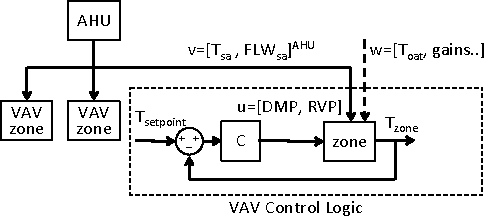
\includegraphics[width=0.45\textwidth]{./figs/ahudiagram.pdf}
                \caption{AHU and VAV configuration. On the right, the VAV control logic is represented. $T_{zone}$ is kept around the $T_{setpoint}$ by the control inputs $u=[DMP, RVP]$. $T_{zone}$ it is also influenced by parameters controlled by the AHU $(v=[T_{sa}, FLW_{sa}]^{AHU}$)  and external disturbances w=[$T_{oat}$, internal gains …].}
                \label{fig:ahudiagram}
\end{figure}

%\input{outline}
\section{Results With Existing Methods}

Techniques commonly employed to detect relationships in data streams include: correlation of raw data ~\cite{koc2014comparison}, correlation of transformed data ~\cite{EMD}, principal component analysis (PCA) and clustering ~\cite{narayanaswamy2014data,hong2013towards}, statistical process control ~\cite{wheeler1992understanding}, and model-based system identification (i.e., building a model by looking for the best fit from a single VAV and alternative AHU data). Preliminary analysis of the building dataset tested conventional correlation methods to find relationships between AHU and the corresponding VAV boxes. Table 1 shows an example of these coefficients. Results show very poor correlation. Desired values inside the bold boxes should be higher, in absolute value, than the corresponding values in the other rows. The same test was repeated with data resampled at 5 min, 15 min and daily, yielding similar results. Thus, this method does not allow identifying which VAV boxes are connected to which AHU.

\begin{table}[ht]\scriptsize
 \caption{Correlation matrix (showing raw data from two AHU and two VAV boxes). Data from May 28 to July 14 2015, resampled at daily rate. }
 \label{tab:corr}
%\centering
%\begin{tabular}{|c{0.5cm}|c{0.5cm}|c{0.5cm}|c{0.5cm}|c{0.5cm}|c{0.5cm}|c{0.5cm}|c{0.5cm}|}
\begin{tabular*}{0.40\textwidth}{|c|c|c|c|c|c|c|c|}
\hline
\multicolumn{2}{|c|}{} & 
  \multicolumn{3}{|c|}{Example $VAV_{AHU3}$} & \multicolumn{3}{|c|}{Example $VAV_{AHU5}$} \\ \hline
\multicolumn{2}{|c|}{} & $T_{zone}$ & DMP & RVP &  $T_{zone}$ & DMP & RVP \\ \hline
AHU 3 & $T_{sa}$ & -0.06 & 0.06 & 0.11 & -0.11 & 0.24 & 0.29 \\ \hline
AHU 5  & $T_{sa}$ & -0.20 & -0.19 & -0.06 & -0.04 & -0.01 & 0.02 \\ \hline
\end{tabular*}
\end{table}



In contrast to prior research monitoring energy consumption ~\cite{EMD}, the variable measured in this test are pressures, temperatures, flows and actuator positions, which show delayed and attenuated responses to changes in input variables, thus reducing correlation. Further, AHU and VAV boxes/zones are physically distant (differently from ~\cite{koc2014comparison}), and variables in the latter are significantly influenced by additional measured and non-measured disturbances (Figure~\ref{fig:ahudiagram}). For this reason, sensor values show a small signal to noise ratio. In addition, sensor readings are frequently constrained between physical limits (e.g. max damper position) and kept around setpoints by nested control loops. Also, cross-talk between systems (i.e., zones might influence each other) and similarity in the way different AHU are controlled (setpoints and daily behavior are similar) make correlation of raw data ineffective.
Next, we constructed feature vectors for the data of each VAV. Features included were: Tzone, DMP, RVP, Tsetpoint, measured flow (FLW), flow setpoint (FWS), day of the week, time of the day. PCA was applied to these feature vectors to identify the two principal components and correlate them to the Tsa. Unfortunately, results of this analysis are not very different from what obtained with raw data (Table 2). Again, this method was ineffective in inferring the relationship investigated.


\begin{table}[ht]\scriptsize
 \caption{ Correlation matrix (showing 2 principal components of VAV data and two AHU). Data from May 28 to July 14 2015}
 \label{tab:pca}
%\centering
%\begin{tabular}{|c{0.5cm}|c{0.5cm}|c{0.5cm}|c{0.5cm}|c{0.5cm}|c{0.5cm}|c{0.5cm}|c{0.5cm}|}
\begin{tabular*}{0.40\textwidth}{|c|c|c|c|c|c|}
\hline
\multicolumn{2}{|c|}{} & 
  \multicolumn{2}{|c|}{Example $VAV_{AHU3}$} & \multicolumn{2}{|c|}{Example $VAV_{AHU5}$} \\ \hline
\multicolumn{2}{|c|}{} & $\lambda_1$ & $\lambda_2$ & $\lambda_1$ &  $\lambda_2$ \\ \hline
AHU 3 & $T_{sa}$ & 0.12 & 0.12 & 0.20 & 0.09  \\ \hline
AHU 5  & $T_{sa}$ & -0.12 & -0.15 & -0.04 & -0.05  \\ \hline
\end{tabular*}
\end{table}


Finally, we tested a completely different and novel approach involving system identification (SID) techniques, which are used in control engineering to find a mathematical relationship (model) between inputs and outputs variables in an observed system [5]. A physics-inspired black-box dynamical model was constructed to predict Tzone, based on the available sensor data: \\

$T_{zone,t} = \beta_1 T_{zone,t-1} + {FLW}_t * \sum\limits_{t}^{t-k} \beta_{2i}{RVP}_i + \beta_3 {FLW}_t * T_{sa,t}^{AHU} + \beta_4 * T_{oat,t}$

where variable names are defined above, $\beta_i$ are the statistical coefficients, and t stands for time. The equation is in the form of an autoregressive (AR) time series model with exogenous inputs and interactive effects (some variables are multiplied). The term with the sum represents the lag in the effect of the reheat valve. The model is based detailed physical knowledge of the heat transfer processes in VAV boxes. Note that all the variables in this equation belong to the VAV with the exception of ($T_{sa,t}^{AHU}$), that represents the supply air temperature controlled by the AHU at time t. The idea is that using the $T_{sa,t}^{AHU}$ from the AHU actually connected to each VAV would improve the model fit. Both linear regression and lasso ~\cite{tibshirani1996regression} were used to fit the model over 15-min resampled data. While the model fit the data very well (R2=76-95\% depending on the zone), it failed to capture the difference in AHU. Plugging in different $T_{sa,t}^{AHU}$ did not change the fit of the model as we had expected. We reasoned that the main cause of this is that the majority of the variation in the output variable $T_{zone,t}$ is captured by the first term of the model (zone temperature at the previous time step) and the remaining $\beta_i$  coefficients are relatively small. With the calculated coefficients, the input variable $T_{sa,t}^{AHU}$ would have to change by more than 20 °F to produce measurable effects in the output variable. Such large temperature differential never occurs spontaneously in our recorded data, and if artificially produced would seriously compromise occupants’ comfort. Nevertheless, this prompted us to explore the idea of actively perturbing the building to measure system response.

\section{Methodology}

The concept underlying the proposed methodology is that by arbitrarily perturbing an AHU we can generate a distinguishable signal in the connected VAV boxes. In practice, by changing dramatically the supply air temperature in an AHU (input), the VAV box will respond by changing some controlled variables (reaheat and damper position) to maintain the temperature setpoint. However, if despite saturation of actuators (damper or reheat valve completely open or close) the system cannot keep up with zone cooling/heating load, the zone temperature ($T_{zone}$) will be affected and change. The AHU supply air temperature was chosen over the AHU flow rate as it is practically easier to tune. Also significantly perturbing flow rates might provide insufficient ventilation or damage the ducts due to high pressure. During the experiment, care was taken in ensuring that the perturbation had no impact on occupant comfort. To do so, while creating an overall large perturbation, the temperature setpoint for the supply air in the AHU was set one day to 52F (cold mode) and the following day to 60F (hot mode), whereby the normal setpoint for a week-day was 57F. Since thermal systems have a significant response lag, the perturbation was sustained for a full day in each mode. To reduce the noise in the data, knowing that VAV variables have little correlation with time of the day (result found while using the other methods), we resampled the data in daily intervals. Average daily values for RVP, DMP and $T_{zone}$ are still meaningful indicator of system behavior.
The algorithm took the following steps:

\begin{enumerate}
\item Perturb one AHU at the time for two consecutive weekdays, one day in cold mode and one day in hot mode. 
\item Collect data for each VAV for the following sensors: RVP, Tzone, DMP. 
\item Re-sample data to obtain daily averages.
\item For each daily average, label the data as belonging to a baseline weekday (WD), cold day, or hot day, for each perturbed AHU (ColdAHU2 would mean cold period for AHU 2). Each VAV data stream will have periods for all AHU perturbations.
\item Standardize each stream of data to have mean =0 and standard deviation = 1.
\item For each VAV and each period combine data into average daily vectors of the form [RVP, DMP, Tzone].
\item Filter out vector elements that show a response value with opposite sign compared to physical intuition (e.g. a cold perturbation that reduced reheat)
\item For each VAV and each couple of AHU perturbations, calculate the Euclidian distance between hot and cold vectors. At the end of this step each zone will have a metric for each AHU hot-cold perturbation.
\item For each VAV take a vote to select the AHU whose perturbation has a highest metric (produced a larger difference in sensor vectors). The AHU selected with this method is expected to be associated with that VAV box.
One important intuition here was that evaluating a metric for each VAV box across all the perturbation periods would provide better results than assigning the zone to an AHU for each perturbation. 
\end{enumerate}


\section{Results}

%\begin{figure}[h!]
%\centering
%                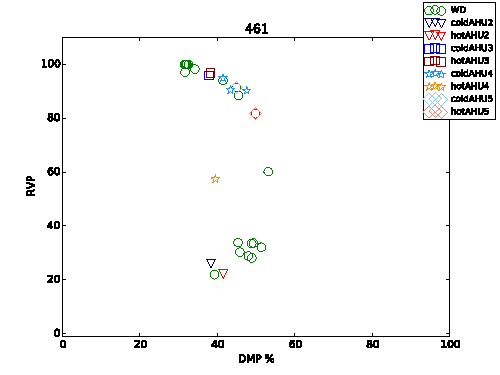
\includegraphics[width=0.45\textwidth,height=2.0in]{./figs/incorrectzone.pdf}
%                \caption{A Zone incorrectly classified by our methodology. Results projected in 2D}
%                \label{fig:incorrectzone}
%\end{figure}
%
%
%\begin{figure*}[ht!]
%\centering
%                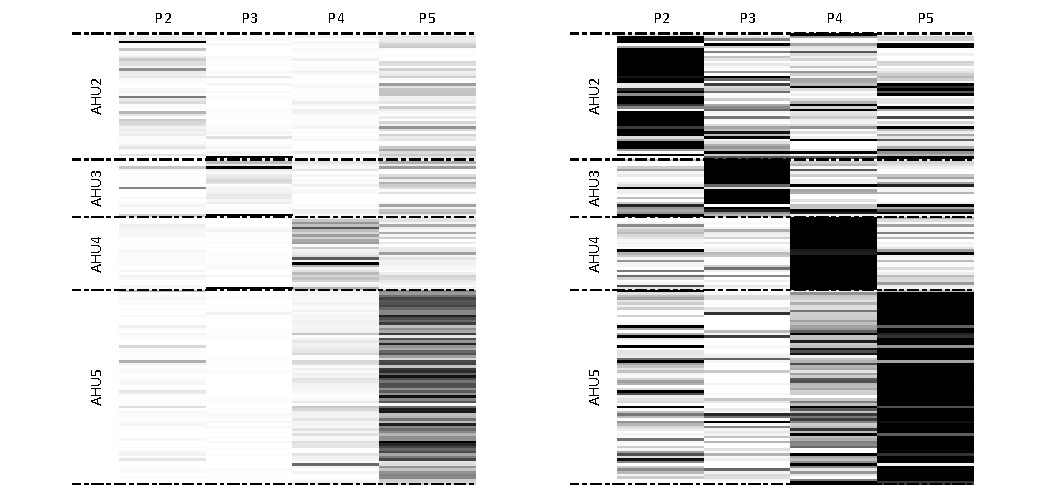
\includegraphics[width=0.90\textwidth,height=2.0in]{./figs/heatmap.pdf}
%                \caption{Heatmap}
%                \label{fig:heatmap}
%\end{figure*}

\begin{figure*}[ht!]
\centering
        \begin{subfigure}{0.30\textwidth}
                \centering
                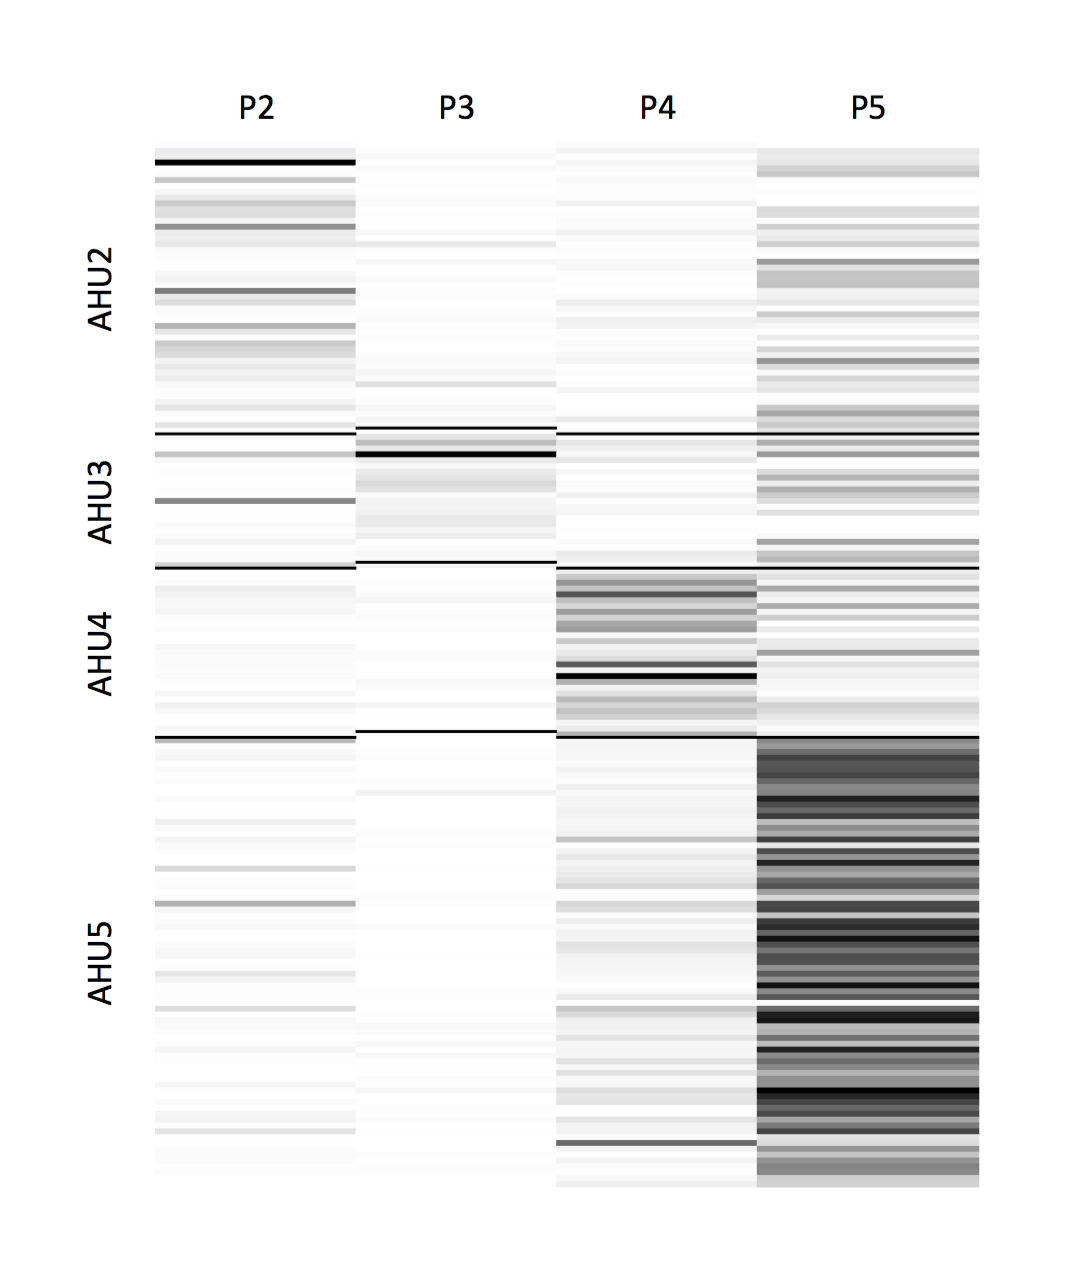
\includegraphics[width=\textwidth,height=2.0in]{./figs/columnnormalized.png}
                \caption{Treating each perturbation as a standalone experiment}
                \label{fig:columnnormalized}
        \end{subfigure}
        \hfill
        \begin{subfigure}{0.30\textwidth}
                \centering
                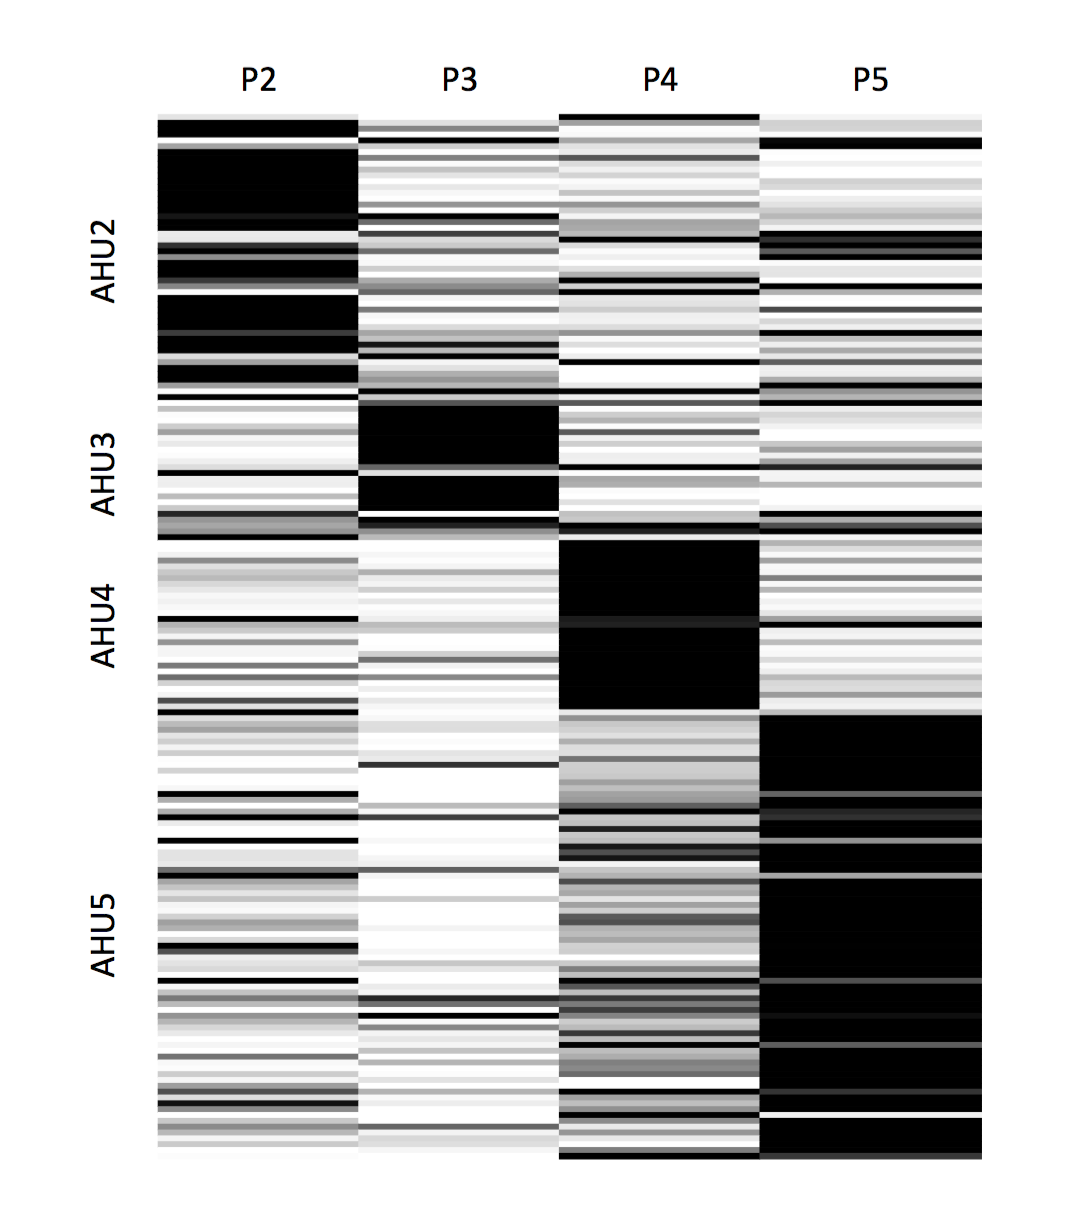
\includegraphics[width=\textwidth,height=2.0in]{./figs/rownormalized.png}
                \caption{Advantages of using a voting method}
                \label{fig:rownormalized}
        \end{subfigure}
        \hfill
                \begin{subfigure}{0.30\textwidth}
                \centering
                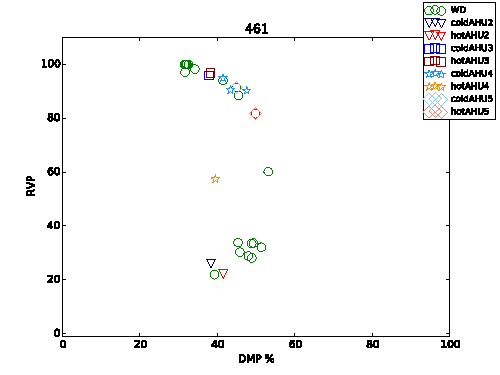
\includegraphics[width=\textwidth,height=2.0in]{./figs/incorrectzone.pdf}
                \caption{A zone incorrectly classified by our methodology. Results projected in 2D}
                \label{fig:incorrectzone}
        \end{subfigure}
\caption{Overview of perturbation statistics across all zones in a building}
\label{fig:active-learning}
\end{figure*}

The proposed methodology was applied to the building explored with the other methods. The results were encouraging, and the method correctly identified the relationship between VAV box and AHU in 79\% of the cases. There were three main groups of rooms that were incorrectly classified: 1) VAVs that showed no response to any perturbation, 2) VAVs that had a unexpected behavior, such as counter-intuitive responses to perturbations, 3) VAVs that responded more strongly to the perturbation of the ‘wrong’ AHU.
For instance Zone 308 (not shown here for brevity) presents a very tight distribution of variables, as DAM is at its minimum, and daily average RVP changes very little during all the periods. Further analysis of this case reveals very frequent oscillations (about 20 cycles per days) of RVP ranging between 0\% and 40\%. It is very likely that the control loop is out of tune for this room. This is likely the reason why the perturbation has no visible effect on the data. This is a misclassification of the first kind.

\begin{table}[ht]\scriptsize
 \caption{ Comparison of accuracy of the voting method and the independent scoring method}
 \label{tab:results}
\begin{tabular*}{0.40\textwidth}{|c|c|c|c|}
\hline
Accuracy/Precision & \multicolumn{2}{|c|}{Independent classification} & Voting \\ \hline
& Threshold=0 & Threshold=2 S.D & Max Value  \\ \hline
AHU 2 &	39\% / 31\% &	78\% / 68 \% &	85\% / 77\% \\
AHU 3 &	35\% / 16\% &	92\% / 85\% &	94\% / 77\% \\
AHU 4 &	22\% / 17\% &	92\% / 77\% &	92\% / 69 \% \\
AHU 5 &	48\% / 45\% &	80\% / 100\% &	86\% / 85\% \\ \hline
\end{tabular*}
\end{table}



On the other hand, zone 461 (Figure 2) shows a very wide distribution of points. The room seem subjected to large unmeasured disturbances. Some baseline weekdays reach max RVP (~100\%), while others use only a fraction of reheat (10-30\%). These unknown factors probably had a larger effect compared to the perturbation, causing the room to be misclassified (type 2).
The effects of adopting a voting system compared to scoring each perturbation individually can be seen in Table 3. The classification of each AHU individually, based on its corresponding perturbation, requires defining a threshold to compare the calculated metric to. Choosing the right threshold is challenging and hard to generalize. In Figure 3 each line represents a VAV box sorted by ground-truth AHU, while each column represents a perturbation of an AHU. The color in each cell is shaded proportionally to the value of the calculated metric, normalized by column. Darker values represent higher metric values and are used to associate the VAV box to the perturbed AHU. It is clear from the figure that each perturbation produces responses in multiple VAV boxes, some of which are not associated with the correct AHU. Choosing a threshold corresponds to choosing a min shade of grey that triggers the association with the AHU currently perturbed. Further, Figure 3 shows that perturbation 3 and perturbation 5 (in column) require a very different threshold to correctly classify the corresponding VAVs. In contrast, Figure 4 illustrates the clearer heat map generated with voting. Dark areas are more clearly defined and it is visually easier to identify which VAV boxes are associated to the AHUs.
In addition, if a room is classified in different ways under separate perturbations (e.g. belonging to two AHUs) then the classification conflict needs to be resolved. When a voting system is adopted, a room is classified in a univocal way. In Table 3 we show the accuracy of the independent classification with two thresholds and the voting method 



\section{Conclusion and Future Work}

In this paper we present a novel algorithm to infer relationships between HVAC components of large commercial buildings. We show that due to the characteristics of the data (response lags, nested control loops, tight variable boundaries) other common techniques are not effective in this context. The new algorithm utilizes perturbations of AHU variables and guarantees that the building zones remain within comfort. The method was applied to an existing building and its results, being able to identify the relationship correctly in ~80\% of the cases.

There are three main directions of research we would like to explore in the future. First, we would like to explore how our technique generalizes to other buildings, where zones may have different sensors, setpoints and control loops. Second, we would like to explore whether we can discover relationships between subsystems like the air handling units and variable air volume units without having to introduce a large perturbation to the air handling unit. We may be able to utilize milder perturbations like daily occupant cycles, and techniques from statistical process control to infer the same relationships. Finally, a useful future direction of research is to quantify the amount of cross-talk between zones. The heat exchange between zones with common doors, passageways, etc introduce errors into any single-zone heat exchange analysis, and its identification and quantification could lead to more efficient and better designed control loops. 

%\input{outline2}
%\input{eval}
%\input{type}
%\input{casestudy}
%\input{apps}
%\input{evaluation}
%\input{application}
%\section{Results With Existing Methods}

Techniques commonly employed to detect relationships in data streams include: correlation of raw data ~\cite{koc2014comparison}, correlation of transformed data ~\cite{EMD}, principal component analysis (PCA) and clustering ~\cite{narayanaswamy2014data,hong2013towards}, statistical process control ~\cite{wheeler1992understanding}, and model-based system identification (i.e., building a model by looking for the best fit from a single VAV and alternative AHU data). Preliminary analysis of the building dataset tested conventional correlation methods to find relationships between AHU and the corresponding VAV boxes. Table 1 shows an example of these coefficients. Results show very poor correlation. Desired values inside the bold boxes should be higher, in absolute value, than the corresponding values in the other rows. The same test was repeated with data resampled at 5 min, 15 min and daily, yielding similar results. Thus, this method does not allow identifying which VAV boxes are connected to which AHU.

\begin{table}[ht]\scriptsize
 \caption{Correlation matrix (showing raw data from two AHU and two VAV boxes). Data from May 28 to July 14 2015, resampled at daily rate. }
 \label{tab:corr}
%\centering
%\begin{tabular}{|c{0.5cm}|c{0.5cm}|c{0.5cm}|c{0.5cm}|c{0.5cm}|c{0.5cm}|c{0.5cm}|c{0.5cm}|}
\begin{tabular*}{0.40\textwidth}{|c|c|c|c|c|c|c|c|}
\hline
\multicolumn{2}{|c|}{} & 
  \multicolumn{3}{|c|}{Example $VAV_{AHU3}$} & \multicolumn{3}{|c|}{Example $VAV_{AHU5}$} \\ \hline
\multicolumn{2}{|c|}{} & $T_{zone}$ & DMP & RVP &  $T_{zone}$ & DMP & RVP \\ \hline
AHU 3 & $T_{sa}$ & -0.06 & 0.06 & 0.11 & -0.11 & 0.24 & 0.29 \\ \hline
AHU 5  & $T_{sa}$ & -0.20 & -0.19 & -0.06 & -0.04 & -0.01 & 0.02 \\ \hline
\end{tabular*}
\end{table}



In contrast to prior research monitoring energy consumption ~\cite{EMD}, the variable measured in this test are pressures, temperatures, flows and actuator positions, which show delayed and attenuated responses to changes in input variables, thus reducing correlation. Further, AHU and VAV boxes/zones are physically distant (differently from ~\cite{koc2014comparison}), and variables in the latter are significantly influenced by additional measured and non-measured disturbances (Figure~\ref{fig:ahudiagram}). For this reason, sensor values show a small signal to noise ratio. In addition, sensor readings are frequently constrained between physical limits (e.g. max damper position) and kept around setpoints by nested control loops. Also, cross-talk between systems (i.e., zones might influence each other) and similarity in the way different AHU are controlled (setpoints and daily behavior are similar) make correlation of raw data ineffective.
Next, we constructed feature vectors for the data of each VAV. Features included were: Tzone, DMP, RVP, Tsetpoint, measured flow (FLW), flow setpoint (FWS), day of the week, time of the day. PCA was applied to these feature vectors to identify the two principal components and correlate them to the Tsa. Unfortunately, results of this analysis are not very different from what obtained with raw data (Table 2). Again, this method was ineffective in inferring the relationship investigated.


\begin{table}[ht]\scriptsize
 \caption{ Correlation matrix (showing 2 principal components of VAV data and two AHU). Data from May 28 to July 14 2015}
 \label{tab:pca}
%\centering
%\begin{tabular}{|c{0.5cm}|c{0.5cm}|c{0.5cm}|c{0.5cm}|c{0.5cm}|c{0.5cm}|c{0.5cm}|c{0.5cm}|}
\begin{tabular*}{0.40\textwidth}{|c|c|c|c|c|c|}
\hline
\multicolumn{2}{|c|}{} & 
  \multicolumn{2}{|c|}{Example $VAV_{AHU3}$} & \multicolumn{2}{|c|}{Example $VAV_{AHU5}$} \\ \hline
\multicolumn{2}{|c|}{} & $\lambda_1$ & $\lambda_2$ & $\lambda_1$ &  $\lambda_2$ \\ \hline
AHU 3 & $T_{sa}$ & 0.12 & 0.12 & 0.20 & 0.09  \\ \hline
AHU 5  & $T_{sa}$ & -0.12 & -0.15 & -0.04 & -0.05  \\ \hline
\end{tabular*}
\end{table}


Finally, we tested a completely different and novel approach involving system identification (SID) techniques, which are used in control engineering to find a mathematical relationship (model) between inputs and outputs variables in an observed system [5]. A physics-inspired black-box dynamical model was constructed to predict Tzone, based on the available sensor data: \\

$T_{zone,t} = \beta_1 T_{zone,t-1} + {FLW}_t * \sum\limits_{t}^{t-k} \beta_{2i}{RVP}_i + \beta_3 {FLW}_t * T_{sa,t}^{AHU} + \beta_4 * T_{oat,t}$

where variable names are defined above, $\beta_i$ are the statistical coefficients, and t stands for time. The equation is in the form of an autoregressive (AR) time series model with exogenous inputs and interactive effects (some variables are multiplied). The term with the sum represents the lag in the effect of the reheat valve. The model is based detailed physical knowledge of the heat transfer processes in VAV boxes. Note that all the variables in this equation belong to the VAV with the exception of ($T_{sa,t}^{AHU}$), that represents the supply air temperature controlled by the AHU at time t. The idea is that using the $T_{sa,t}^{AHU}$ from the AHU actually connected to each VAV would improve the model fit. Both linear regression and lasso ~\cite{tibshirani1996regression} were used to fit the model over 15-min resampled data. While the model fit the data very well (R2=76-95\% depending on the zone), it failed to capture the difference in AHU. Plugging in different $T_{sa,t}^{AHU}$ did not change the fit of the model as we had expected. We reasoned that the main cause of this is that the majority of the variation in the output variable $T_{zone,t}$ is captured by the first term of the model (zone temperature at the previous time step) and the remaining $\beta_i$  coefficients are relatively small. With the calculated coefficients, the input variable $T_{sa,t}^{AHU}$ would have to change by more than 20 °F to produce measurable effects in the output variable. Such large temperature differential never occurs spontaneously in our recorded data, and if artificially produced would seriously compromise occupants’ comfort. Nevertheless, this prompted us to explore the idea of actively perturbing the building to measure system response.

%\input{discussion}
%\section{Conclusion and Future Work}

In this paper we present a novel algorithm to infer relationships between HVAC components of large commercial buildings. We show that due to the characteristics of the data (response lags, nested control loops, tight variable boundaries) other common techniques are not effective in this context. The new algorithm utilizes perturbations of AHU variables and guarantees that the building zones remain within comfort. The method was applied to an existing building and its results, being able to identify the relationship correctly in ~80\% of the cases.

There are three main directions of research we would like to explore in the future. First, we would like to explore how our technique generalizes to other buildings, where zones may have different sensors, setpoints and control loops. Second, we would like to explore whether we can discover relationships between subsystems like the air handling units and variable air volume units without having to introduce a large perturbation to the air handling unit. We may be able to utilize milder perturbations like daily occupant cycles, and techniques from statistical process control to infer the same relationships. Finally, a useful future direction of research is to quantify the amount of cross-talk between zones. The heat exchange between zones with common doors, passageways, etc introduce errors into any single-zone heat exchange analysis, and its identification and quantification could lead to more efficient and better designed control loops. 


% \balance
\bibliographystyle{abbrv}
\footnotesize
\bibliography{sigproc}  % sigproc.bib is the name of the Bibliography in this case
\end{document}
